% Copyright (c) 2026 CorrectBrain
% SPDX-License-Identifier: MIT

\PassOptionsToPackage{dvipsnames,svgnames,x11names}{xcolor}
\documentclass[tikz,border=8pt]{standalone}
\usetikzlibrary{arrows.meta,positioning,calc,shapes,shadows,decorations.pathmorphing,shapes.geometric,backgrounds,decorations.markings,decorations.pathreplacing,decorations.text,fit,shapes.misc,shapes.arrows,matrix,bending,3d,chains,intersections,shapes.symbols,svg.path,shapes.multipart,snakes,shapes.callouts,angles,quotes,fadings,shadows.blur,patterns,patterns.meta}
\usepackage{amsmath}
\usepackage{amssymb}
\usepackage{fontawesome5}

\providecolor{gold}{RGB}{212,175,55}
\providecolor{silver}{RGB}{192,192,192}
\providecolor{bronze}{RGB}{205,127,50}
\providecolor{darkblue}{RGB}{0,0,139}
\providecolor{lightblue}{RGB}{173,216,230}
\providecolor{darkgreen}{RGB}{0,100,0}
\providecolor{lightgreen}{RGB}{144,238,144}
\providecolor{darkred}{RGB}{139,0,0}
\providecolor{navy}{RGB}{0,0,128}
\providecolor{skyblue}{RGB}{135,206,235}
\providecolor{beige}{RGB}{245,245,220}
\providecolor{cream}{RGB}{255,253,208}

% --- COLOR DEFINITIONS (SLATE & MODERN PALETTE) ---
\definecolor{slate-50}{RGB}{248, 250, 252}
\definecolor{slate-100}{RGB}{241, 245, 249}
\definecolor{slate-200}{RGB}{226, 232, 240}
\definecolor{slate-300}{RGB}{203, 213, 225}
\definecolor{slate-400}{RGB}{148, 163, 184}
\definecolor{slate-500}{RGB}{100, 116, 139}
\definecolor{slate-600}{RGB}{71, 85, 105}
\definecolor{slate-700}{RGB}{51, 65, 85}
\definecolor{slate-800}{RGB}{30, 41, 59}
\definecolor{slate-900}{RGB}{15, 23, 42}

\definecolor{gray-900}{RGB}{24, 24, 27}
\definecolor{codeheader}{RGB}{39, 39, 42}

% Syntax Highlighting
\definecolor{tagcol}{RGB}{244, 63, 94}
\definecolor{attrcol}{RGB}{251, 146, 60}
\definecolor{strcol}{RGB}{74, 222, 128}

% Mac Window Controls
\definecolor{macred}{RGB}{255, 95, 86}
\definecolor{macyellow}{RGB}{255, 189, 46}
\definecolor{macgreen}{RGB}{39, 201, 63}

% Logic Flow Accents
\definecolor{accentblue}{RGB}{2, 132, 199}
\definecolor{accentpurple}{RGB}{124, 58, 237}
\definecolor{accentgreen}{RGB}{22, 163, 74}
\definecolor{accentred}{RGB}{225, 29, 72}

\begin{document}
\begin{tikzpicture}[x=1cm, y=1cm]

% 1. Pure White Canvas Background (Strict Blueprint Compliance)
\fill[white] (-15.0, -25.0) rectangle (15.0, 11.5);

% --- HEADER SECTION ---
\node[font=\Huge\bfseries\color{slate-800}] at (0, 10) {Capability \& Spatial Negotiation Algorithm};
\node[font=\Large\color{slate-500}, align=center, text width=24cm] at (0, 9) {How \texttt{<picture>} constructs a multi-dimensional software evaluation tree using \texttt{media} and \texttt{type} attributes.};

% --- TOP SECTION: MAC-STYLE IDE & GLASSMORPHISM THEORY PANEL ---

% 1. IDE Code Window (-12.5, 1) to (-1.0, 8)
\path[fill=gray-900, rounded corners=8pt, blur shadow={shadow opacity=40, shadow yshift=-3mm, shadow blur steps=10}] (-12.5, 1) rectangle (-1.0, 8);

% Window Title Bar
\path[fill=codeheader, rounded corners=8pt] (-12.5, 7.3) rectangle (-1.0, 8);
\path[fill=codeheader] (-12.5, 7.3) rectangle (-1.0, 7.5);
\draw[draw=slate-700, line width=0.5pt] (-12.5, 7.3) -- (-1.0, 7.3);

% Window Control Buttons
\fill[macred] (-12.0, 7.65) circle (3.2pt);
\fill[macyellow] (-11.6, 7.65) circle (3.2pt);
\fill[macgreen] (-11.2, 7.65) circle (3.2pt);
\node[font=\footnotesize\bfseries\color{slate-300}, anchor=center] at (-6.75, 7.65) {\faCode \quad HTML Structure};

% HTML Code Lines (Character-for-Character Preserved)
\node[font=\ttfamily\small, anchor=west] at (-12.0, 6.7) {\color{tagcol}{<picture>}};
\node[font=\ttfamily\small, anchor=west] at (-11.5, 6.0) {\color{tagcol}{<source} \color{attrcol}{media=}\color{strcol}{"(min-width: 800px)"} \color{attrcol}{type=}\color{strcol}{"image/avif"}};
\node[font=\ttfamily\small, anchor=west] at (-10.5, 5.4) {\color{attrcol}{srcset=}\color{strcol}{"desktop.avif"}\color{tagcol}{>}};
\node[font=\ttfamily\small, anchor=west] at (-11.5, 4.7) {\color{tagcol}{<source} \color{attrcol}{media=}\color{strcol}{"(min-width: 800px)"} \color{attrcol}{type=}\color{strcol}{"image/webp"}};
\node[font=\ttfamily\small, anchor=west] at (-10.5, 4.1) {\color{attrcol}{srcset=}\color{strcol}{"desktop.webp"}\color{tagcol}{>}};
\node[font=\ttfamily\small, anchor=west] at (-11.5, 3.4) {\color{tagcol}{<img} \color{attrcol}{src=}\color{strcol}{"mobile.jpg"} \color{attrcol}{alt=}\color{strcol}{"..."}\color{tagcol}{>}};
\node[font=\ttfamily\small, anchor=west] at (-12.0, 2.7) {\color{tagcol}{</picture>}};

% 2. Glassmorphism Theory Panel (0.0, 1) to (12.5, 8)
\path[top color=white, bottom color=slate-50, draw=slate-300, line width=0.5pt, rounded corners=8pt, blur shadow={shadow opacity=15, shadow yshift=-2mm, shadow blur steps=8}] (0.0, 1) rectangle (12.5, 8);
\node[font=\large\bfseries\color{slate-800}, anchor=west] at (0.5, 7.35) {\faCogs \quad Software Version Dependency};
\draw[draw=slate-200, line width=0.5pt] (0.5, 6.9) -- (12.0, 6.9);
\node[font=\small\color{slate-800}, anchor=north west, text width=11.8cm, align=left] at (0.4, 6.6) {
    The inclusion of \texttt{type} inherently couples the layout to the \textbf{browser's software version}.\\[1.5ex]
    Older software engines (e.g., Safari 13, IE11) lack the decoders for modern formats like AVIF or WebP. When the parser evaluates the \texttt{type} attribute, it acts as a boolean capability check.\\[1.5ex]
    \textbf{If capability check fails (False):} The algorithm abandons that \texttt{<source>} node entirely and proceeds down the DOM tree, regardless of whether the spatial \texttt{media} query was true.
};

% --- BROWSER ENGINE BOUNDING ENVIRONMENT ---
\draw[draw=slate-300, fill=slate-50, rounded corners=12pt, dashed, line width=1pt] (-14.0, -24.0) rectangle (13.5, -0.5);
\node[fill=slate-200, draw=slate-300, line width=0.5pt, rounded corners=4pt, font=\scriptsize\bfseries\color{slate-700}, anchor=west, inner sep=6pt] at (-13.5, -1.2) {\faCogs \quad Browser Layout \& Capability Evaluator (e.g., Blink/WebKit)};
\node[font=\Large\bfseries\color{slate-800}] at (-4.0, -2.5) {Top-to-Bottom Engine Evaluation Logic};

% --- FLOWCHART STYLES ---
\tikzstyle{process} = [draw=slate-300, fill=white, line width=1pt, text=slate-800, font=\small\bfseries, rounded corners=6pt, inner sep=6pt, text width=4.2cm, align=center, blur shadow={shadow opacity=12}]
\tikzstyle{decision-media} = [shape=diamond, aspect=2.0, top color=white, bottom color=accentblue!12, draw=accentblue!80, line width=1.2pt, text=slate-800, font=\footnotesize\bfseries, inner sep=4pt, text width=3.8cm, align=center, blur shadow={shadow opacity=15}]
\tikzstyle{decision-type} = [shape=diamond, aspect=2.0, top color=white, bottom color=accentpurple!12, draw=accentpurple!80, line width=1.2pt, text=slate-800, font=\footnotesize\bfseries, inner sep=4pt, text width=3.8cm, align=center, blur shadow={shadow opacity=15}]
\tikzstyle{result-avif} = [preaction={draw=accentgreen, line width=4.5pt, opacity=0.35, rounded corners=6pt}, draw=accentgreen!80!black, fill=accentgreen, text=white, font=\small\bfseries, rounded corners=6pt, inner sep=6pt, text width=3.8cm, align=center, blur shadow={shadow opacity=20}]
\tikzstyle{result-webp} = [preaction={draw=accentblue, line width=4.5pt, opacity=0.35, rounded corners=6pt}, draw=accentblue!80!black, fill=accentblue, text=white, font=\small\bfseries, rounded corners=6pt, inner sep=6pt, text width=3.8cm, align=center, blur shadow={shadow opacity=20}]
\tikzstyle{result-jpg} = [preaction={draw=accentred, line width=4.5pt, opacity=0.35, rounded corners=6pt}, draw=accentred!80!black, fill=accentred, text=white, font=\small\bfseries, rounded corners=6pt, inner sep=6pt, text width=3.8cm, align=center, blur shadow={shadow opacity=20}]
\tikzstyle{arrow} = [-Stealth=3mm, thick, color=slate-600, rounded corners=4pt]

% --- FLOWCHART NODES (SYMMETRICAL TRUNK LAYOUT) ---

% Start Node
\node[draw=slate-800, fill=slate-800, text=white, font=\small\bfseries, rounded corners=6pt, inner sep=6pt, text width=4.2cm, align=center, blur shadow={shadow opacity=20}] (start) at (-4.0, -3.8) {Begin \texttt{<picture>} Parse};

% Source 1 Tier
\node[process] (s1) at (-4.0, -5.5) {\texttt{<source>} 1 \\ \textcolor{slate-500}{\footnotesize AVIF for Desktop}};
\node[decision-media] (d1m) at (-8.5, -9.0) {Media matches?\\ \textcolor{slate-500}{\scriptsize (min-width: 800px)}};
\node[decision-type] (d1t) at (1.0, -9.0) {Software supports\\ \texttt{type="image/avif"}?};
\node[result-avif] (r1) at (10.0, -9.0) {\faWifi \ Network Request:\\ \texttt{desktop.avif}};

% Source 2 Tier
\node[process] (s2) at (-4.0, -14.0) {\texttt{<source>} 2 \\ \textcolor{slate-500}{\footnotesize WebP for Desktop}};
\node[decision-media] (d2m) at (-8.5, -17.5) {Media matches?\\ \textcolor{slate-500}{\scriptsize (min-width: 800px)}};
\node[decision-type] (d2t) at (1.0, -17.5) {Software supports\\ \texttt{type="image/webp"}?};
\node[result-webp] (r2) at (10.0, -17.5) {\faWifi \ Network Request:\\ \texttt{desktop.webp}};

% Fallback Tier
\node[draw=accentred, fill=white, line width=1.2pt, text=accentred, font=\small\bfseries, rounded corners=6pt, inner sep=6pt, text width=4.2cm, align=center, blur shadow={shadow opacity=15}] (img) at (-4.0, -22.5) {Fallback \texttt{<img>} \\ \textcolor{slate-500}{\footnotesize JPG for all others}};
\node[result-jpg] (r3) at (10.0, -22.5) {\faWifi \ Network Request:\\ \texttt{mobile.jpg}};

% --- SYMMETRICAL & ORTHOGONAL ROUTING PATHS (ZERO COLLISION) ---

% Start -> Source 1
\draw[arrow] (start) -- (s1);

% Source 1 Evaluation Path (YES)
\draw[arrow] (s1.south) -- (-4.0, -7.0) -| (d1m.north);
\draw[arrow] (d1m.east) -- node[above, fill=slate-50, yshift=2pt, font=\footnotesize\bfseries\color{accentgreen}] {YES (Desktop)} (d1t.west);
\draw[arrow] (d1t.east) -- node[above, fill=slate-50, yshift=2pt, font=\footnotesize\bfseries\color{accentgreen}] {YES (Chrome 85+)} (r1.west);

% Source 1 Failures -> Unified Failure Merge -> Source 2 (NO)
\draw[thick, color=slate-600, rounded corners=4pt] (d1m.south) |- (-4.0, -12.0);
\draw[thick, color=slate-600, rounded corners=4pt] (d1t.south) |- (-4.0, -12.0);
\node[anchor=south, fill=slate-50, font=\footnotesize\bfseries\color{accentred}, inner sep=2pt] at (-6.25, -12.0) {NO (Mobile)};
\node[anchor=south, fill=slate-50, font=\footnotesize\bfseries\color{accentred}, inner sep=2pt] at (-1.5, -12.0) {NO (Older Browser)};
\draw[arrow] (-4.0, -12.0) -- (s2.north);

% Source 2 Evaluation Path (YES)
\draw[arrow] (s2.south) -- (-4.0, -15.5) -| (d2m.north);
\draw[arrow] (d2m.east) -- node[above, fill=slate-50, yshift=2pt, font=\footnotesize\bfseries\color{accentgreen}] {YES (Desktop)} (d2t.west);
\draw[arrow] (d2t.east) -- node[above, fill=slate-50, yshift=2pt, font=\footnotesize\bfseries\color{accentgreen}] {YES (Safari 14+)} (r2.west);

% Source 2 Failures -> Unified Failure Merge -> Fallback <img> (NO)
\draw[thick, color=slate-600, rounded corners=4pt] (d2m.south) |- (-4.0, -20.5);
\draw[thick, color=slate-600, rounded corners=4pt] (d2t.south) |- (-4.0, -20.5);
\node[anchor=south, fill=slate-50, font=\footnotesize\bfseries\color{accentred}, inner sep=2pt] at (-6.25, -20.5) {NO (Mobile)};
\node[anchor=south, fill=slate-50, font=\footnotesize\bfseries\color{accentred}, inner sep=2pt] at (-1.5, -20.5) {NO (IE11)};
\draw[arrow] (-4.0, -20.5) -- (img.north);

% Fallback Execution Path
\draw[arrow] (img.east) -- node[above, fill=slate-50, yshift=2pt, font=\footnotesize\bfseries\color{accentgreen}] {Unconditional (If Reached)} (r3.west);

\end{tikzpicture}
\end{document}
